\documentclass[a4paper,10pt]{article}

\usepackage[brazil]{babel}

\usepackage{array}

\usepackage[portuguese, ruled, linesnumbered]{algorithm2e}

\usepackage{graphicx}
\usepackage{caption}
\usepackage{subcaption}

\usepackage{placeins}
\usepackage{float}

\usepackage{natbib}
 
\usepackage{url}

\usepackage[utf8]{inputenc}

\usepackage{amssymb,fancybox,epsfig,psfrag,amsmath,tabularx}

%%%%%%%%%%%%%%%%%%%%%%%%%%%%%%%%%%%%%%%%%%%%%%%%%%%%%%%%%%%%%%%%%%%%%%%%%%%%%%%%%%%%%%%%%%
%% Margenes
%%%%%%%%%%%%%%%%%%%%%%%%%%%%%%%%%%%%%%%%%%%%%%%%%%%%%%%%%%%%%%%%%%%%%%%%%%%%%%%%%%%%%%%%%%
\usepackage{vmargin}

\setpapersize{A4}
\setmargins{3.0cm}% margen izquierdo
	    {1.5cm}% margen superior
	    {15.0cm}% anchura del texto
	    {23cm}% altura del texto
	    {10pt}% altura de los encabezados
	    {1cm}% espacio entre el texto y los encabezados
	    {10pt}% altura del pie de página
	    {2cm}% espacio entre el texto y el pie de página

%%%%%%%%%%%%%%%%%%%%%%%%%%%%%%%%%%%%%%%%%%%%%%%%%%%%%%%%%%%%%%%%%%%%%%%%%%%%%%%%%%%%%%%%%%
%% Defino estilo de theoremas
%%%%%%%%%%%%%%%%%%%%%%%%%%%%%%%%%%%%%%%%%%%%%%%%%%%%%%%%%%%%%%%%%%%%%%%%%%%%%%%%%%%%%%%%%%
  \usepackage{amsthm}
  
  % Teoremas normales : Funciona bien con todo.
  % % Teoremas normales
%%%%%%%%%%%%%%%%%%%
\theoremstyle{definition}
\newtheorem{proposition}{Proposição}[section]
\newtheorem{theorem}{Teorema}[section]
\newtheorem{lemma}{Lema}[section]
\newtheorem{definition}{Definição}[section]
\newtheorem{conjecture}{Conjectura}[section]
\newtheorem{corollary}{Corolário}[section]

  
  % Teoremas en cajas: Funciona bien con PDFLaTex
  % \usepackage{mdframed}
\newmdtheoremenv[skipabove=\topsep,skipbelow=\topsep]{theoremsqr}{Teorema}[thm]

  
  % Teoremas en cajas aredondadas de colores : Funciona bien con PDFLaTex
  % no quiebra cuadro alltar de pagina
  % exemplo
  % \begin{theorembox}[Titulo del teorema] \label{teo:propor}
  % X 
  % \end{theorembox}  
  % %exemplo
%\begin{theorembox}[Titulo del teorema] \label{teo:propor}
%X 
%\end{theorembox}

\usepackage{etoolbox}% http://ctan.org/pkg/etoolbox
\usepackage{needspace}% http://ctan.org/pkg/needspace


\usepackage{structure/theorems/boiboites} % invoca a boiboites.sty


\newboxedtheorem[boxcolor=gray, 
                 background=gray!15, 
                 titlebackground=gray!5,
                 titleboxcolor = black]
                 {theorembox}{Teorema}{thm}
                 
\AtBeginEnvironment{theorembox}{\Needspace{5\baselineskip}}
                 
\newboxedtheorem[boxcolor=blue, 
                 background=blue!15, 
                 titlebackground=blue!5,
                 titleboxcolor = black]
                 {definitionbox}{Definicion}{thm}

\newboxedtheorem[boxcolor=red, 
                 background=red!15, 
                 titlebackground=red!5,
                 titleboxcolor = black]
                 {corollarybox}{Corolario}{coro}
                 
                 
  
  
  
  %\begin{corollarytcolorbox}{Titulo}{label1}
  % texto  
  % \end{corollarytcolorbox}
  %
  %\begin{theoremtcolorbox}{Titulo}{label2}
  % texto  
  % \end{theoremtcolorbox}
  \usepackage{tcolorbox}
\tcbuselibrary{theorems}

\definecolor{lowgray}{rgb}{0.95,0.95,0.95}

\newcounter{theocount} 
\newcounter{corocount} 

\tcbmaketheorem{theoremtcolorbox}{Teorema}{ colback=lowgray!5,
					    colframe=lowgray!35!black,
					    breakable,                               % this will make the box breaks when the end of the page is reached
					    fonttitle=\bfseries}{theocount}{teo}
					    
\tcbmaketheorem{corollarytcolorbox}{Corolário}{ colback=red!3,
					    colframe=red!30!black!50,
					    breakable,                               % this will make the box breaks when the end of the page is reached
					    fonttitle=\bfseries}{corocount}{coro}

  
  
  
  %http://tex.stackexchange.com/questions/120454/theorem-with-separate-tikz-environments-for-header-and-body

%%%%%%%%%%%%%%%%%%%%%%%%%%%%%%%%%%%%%%%%%%%%%%%%%%%%%%%%%%%%%%%%%%%%%%%%%%%%%%%%%%%%%%%%%%
%%%%%%%%%%%%%%%%%%%%%%%%%%%%%%%%%%%%%%%%%%%%%%%%%%%%%%%%%%%%%%%%%%%%%%%%%%%%%%%%%%%%%%%%%%


%%%%%%%%%%%%%%%%%%%%%%%%%%%%%%%%%%%%%%%%%%%%%%%%%%%%%%%%%%%%%%%%%%%%%%%%%%%%%%%%%%%%%%%%%%
%% Defino bloques de texto con marco y color
%%%%%%%%%%%%%%%%%%%%%%%%%%%%%%%%%%%%%%%%%%%%%%%%%%%%%%%%%%%%%%%%%%%%%%%%%%%%%%%%%%%%%%%%%%

  % textos en cajas de colores
  %example
  %\begin{bclogo}[couleur=blue!30, arrondi=0.1,logo=\bccrayon,ombre=true]{Titulo da caixa}
  % texto qualquer.
  %\end{bclogo}
  \usepackage[tikz]{bclogo}
%example
%\begin{bclogo}[couleur=blue!30, arrondi=0.1,logo=\bccrayon,ombre=true]{Titulo da caixa}
% texto qualquer.
%\end{bclogo}


  
  % Exemplo1
  % \begin{tcolorboxgreycolor}{Titulo}%% {tcolorboxgreen},{tcolorboxbluecolor}
  % texto
  % \end{tcolorboxgreycolor}
  %
  % Exemplo2
  % \begin{tcolorbox}[colback=red!5!white,colframe=red!75!black,title=My Heading]
  % Texto2
  % \end{tcolorbox}
  % Exemplo1
% \begin{tcolorboxgreycolor}{Titulo} %% {tcolorboxgreen},{tcolorboxbluecolor}
% texto
% \end{tcolorboxgreycolor}
%
% Exemplo2
% \begin{tcolorbox}[colback=red!5!white,colframe=red!75!black,title=My Heading]
% Texto2
% \end{tcolorbox}

\usepackage{color}

\usepackage{tcolorbox}
\tcbuselibrary{skins,breakable}
\usetikzlibrary{shadings,shadows}

\definecolor{greycolor}{rgb}{0.1,0.1,0.1}
\definecolor{greencolor}{rgb}{0.1,1,0.1}
\definecolor{darkgreencolor}{HTML}{024103}
\definecolor{darkbluecolor}{HTML}{000A62}


\newenvironment{tcolorboxgreycolor}[1]{%
    \tcolorbox[beamer,%
    noparskip,breakable,
    colback=greycolor!5!white,colframe=greycolor!75!black,%
    title=#1]}%
    {\endtcolorbox}
    
\newenvironment{tcolorboxgreencolor}[1]{%
    \tcolorbox[beamer,%
    noparskip,breakable,
    colback=darkgreencolor!5!white,colframe=darkgreencolor!75!black,%
    title=#1]}%
    {\endtcolorbox}

\newenvironment{tcolorboxbluecolor}[1]{%
    \tcolorbox[beamer,%
    noparskip,breakable,
    colback=darkbluecolor!5!white,colframe=darkbluecolor!75!black,%
    colbacklower=darkbluecolor!75!black,%
    title=#1]}%
    {\endtcolorbox}

  
%%%%%%%%%%%%%%%%%%%%%%%%%%%%%%%%%%%%%%%%%%%%%%%%%%%%%%%%%%%%%%%%%%%%%%%%%%%%%%%%%%%%%%%%%%
%%%%%%%%%%%%%%%%%%%%%%%%%%%%%%%%%%%%%%%%%%%%%%%%%%%%%%%%%%%%%%%%%%%%%%%%%%%%%%%%%%%%%%%%%%


%%%%%%%%%%%%%%%%%%%%%%%%%%%%%%%%%%%%%%%%%%%%%%%%%%%%%%%%%%%%%%%%%%%%%%%%%%%%%%%%%%%%%%%%%%
%% Defino bloques de texto con marco y color
%%%%%%%%%%%%%%%%%%%%%%%%%%%%%%%%%%%%%%%%%%%%%%%%%%%%%%%%%%%%%%%%%%%%%%%%%%%%%%%%%%%%%%%%%%

  % Example
  % \begin{tcolorbox}[tab2,tabularx={X||Y|Y|Y|Y||Y}]
  % Group & One     & Two     & Three    & Four     & Sum      \\\hline\hline
  % Red   & 1000.00 & 2000.00 &  3000.00 &  4000.00 & 10000.00 
  % \end{tcolorbox}
  % 
  % \begin{tcolorbox}[tab2,tabularx={X||Y|Y|Y|Y||Y},title=My table,boxrule=0.5pt]
  % Group & One     & Two     & Three    & Four     & Sum      \\\hline\hline
  % Red   & 1000.00 & 2000.00 &  3000.00 &  4000.00 & 10000.00 
  % \end{tcolorbox}
  % 
  % \begin{tcolorbox}[tab1,tabularx={X||YYYY||Y}]
  % Group & One     & Two     & Three    & Four     & Sum      \\\hline\hline
  % Red   & 1000.00 & 2000.00 &  3000.00 &  4000.00 & 10000.00 
  % \end{tcolorbox}
  
\usepackage{tcolorbox}
\usepackage{tabularx}
\usepackage{array}
\usepackage{colortbl}
\tcbuselibrary{skins}


\newcolumntype{Y}{>{\raggedleft\arraybackslash}X}

\tcbset{tab1/.style={ fonttitle=\bfseries\large,
		      fontupper=\normalsize\sffamily,
		      colback=yellow!10!white,
		      colframe=red!75!black,
		      colbacktitle=red!40!white,
		      coltitle=black,
		      center title,
		      freelance,
		      frame code={\foreach \n in  {north east,north west,south east,south west}
						  {\path [fill=red!75!black] (interior.\n) circle (3mm); };
				},
		      }
	}

\tcbset{tab2/.style={ enhanced,
		      fonttitle=\bfseries,
		      fontupper=\normalsize\sffamily,
		      colback=yellow!10!white,
		      colframe=red!50!black,
		      colbacktitle=red!40!white,
		      coltitle=black,
		      center title
		      }
	}

\tcbset{tabgrey/.style={ enhanced,
		      fonttitle=\bfseries,
		      fontupper=\normalsize\sffamily,
		      colback=black!5!white,
		      colframe=white!50!black,
		      colbacktitle=black!20!white,
		      coltitle=black,
		      center title
		      }
	}	
  
%%%%%%%%%%%%%%%%%%%%%%%%%%%%%%%%%%%%%%%%%%%%%%%%%%%%%%%%%%%%%%%%%%%%%%%%%%%%%%%%%%%%%%%%%%
%%%%%%%%%%%%%%%%%%%%%%%%%%%%%%%%%%%%%%%%%%%%%%%%%%%%%%%%%%%%%%%%%%%%%%%%%%%%%%%%%%%%%%%%%%   

%opening
\title{Cálculo de disparidade entre duas câmeras deslocadas e com um giro de perspectiva }
\author{Fernando Pujaico Rivera}

\begin{document}

\maketitle

\begin{abstract}
Aqui descreverei como obter o mapa de disparidade, mediante a informação proveniente de  duas câmeras 
deslocadas nos 3 eixos e com linhas de visão não paralelas.
\end{abstract}

\section{Introdução}

Este trabalho visa resolver o problema de determinar o mapa de disparidade 
desde a informação fornecida por duas imagens, Imagem 1 e Imagem 2, com pontos de 
coincidência $D_{1p}$ e $D_{2p}$ respetivamente.
Assim, para obter o mapa de disparidade,
se simplificará o problema a que deseja-se determinar a posição de um ponto $P$ 
visto desde as perspectivas das bases canônicas de coordenadas da câmera 1 e da câmera 2.
A Figura \ref{fig:modelosimple} descreve esta situação mais detalhadamente.

Serão considerados dois tipos de bases para os eixos coordenados, teremos a base canônica
e a base não canônica, que denominaremos base natural.
Ambas câmeras terão bases, canônicas ou naturais, com eixos perpendiculares entre sim, e com o ponto $(0,0,0)$ 
sobre as câmeras, independentemente de se a base é canônica ou natural.
Para descrever estas bases, usaremos os elementos $\{+X,+Y,+Z\}$ para denotar a direção 
dos eixos perpendiculares, sendo que existirá uma triada $\{+X,+Y,+Z\}$ para cada 
base canônica e natural.


\begin{figure}[!ht]
\center
 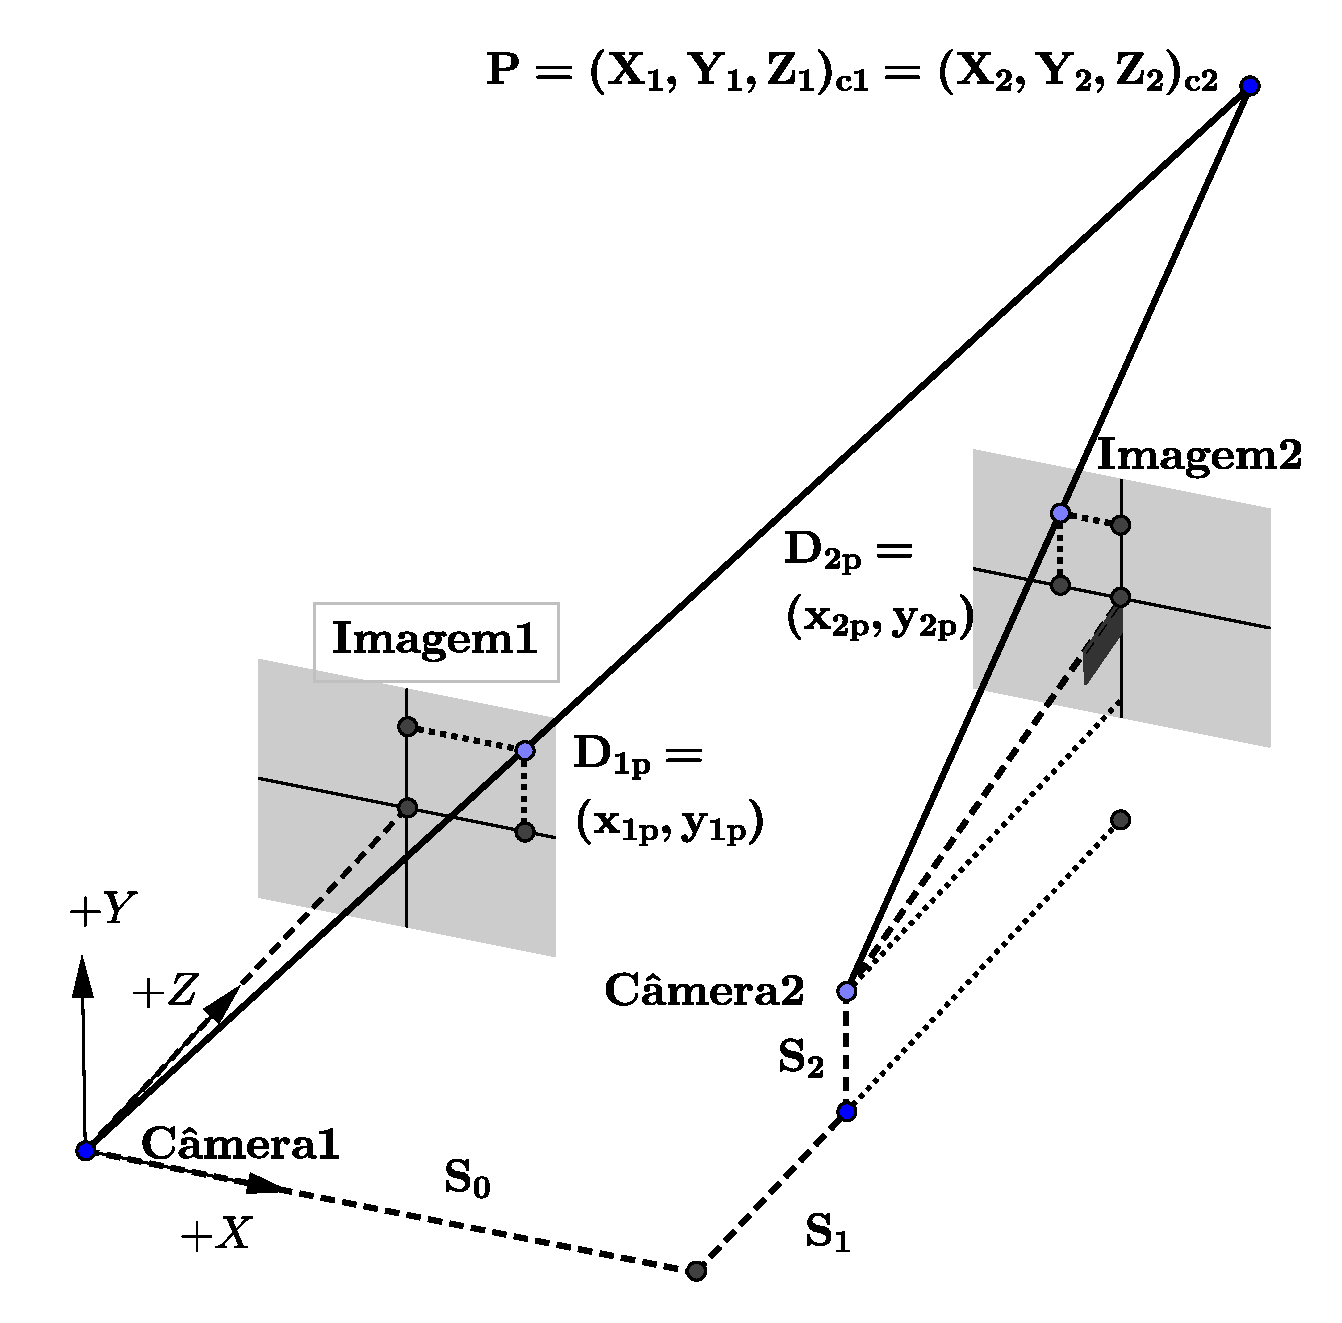
\includegraphics[width=8.0cm]{./images/Modelo.eps}
\caption{Modelo do sistema com duas câmeras deslocadas e com linhas de visão não paralelas.}
\label{fig:modelosimple}
\end{figure} 

Será chamado de base natural da câmera 1, ao eixo $+Z$
apontando perpendicularmente à Imagem 1, o eixo $+X$ apontando a direita da imagem 1 e o eixo $+Y$
apontando para arriba da mesma imagem; para esta câmera será considerado que a base canônica é a mesma da base natural. 

A base natural da câmera 2 terá o eixo $+Z$ apontando perpendicularmente à Imagem 2, 
o eixo $+X$ apontando a direita da imagem 2 e o eixo $+Y$
apontando para arriba da mesma imagem. 
Se considerará que a base natural da câmera 2 é distinta da  base canônica da mesma câmera, de modo que a base canônica da câmera 2 terá os eixos coordenados 
paralelos aos eixos da base canônica da câmera 1.

Em todo este trabalho o uso de uma variável com sub-índice $p$, indicará que o número
que representa a variável usa unidades em pixeis.
De não ser assim, deve-se considerar que a distancia está em metros.

\section{Dados do problema}

\subsection{Dados da câmera e dos arquivos de imagem}
Em todo este trabalho  assume-se que ambas câmeras tem a mesma configuração física,
como a especificada na Figura \ref{fig:camera}. Ali pode-se ver que a imagem é
gerada a uma distancia $h_0$ (em metros) da câmera, formando um angulo reto com a sua linha
de visão, que coincide com o eixo $+Z$ de sua base natural. O ponto de interseção
($I$ na Figura \ref{fig:camera}) está no ponto médio, horizontal e vertical, da imagem.
Será definido como $\alpha$ ao angulo de visão horizontal das câmeras. Como é 
mostrado no Teorema \ref{teo:angulo}, o angulo $\alpha$ cumpre que,
\begin{equation} \label{eq:dat1}
 \frac{W}{h_0}=2~tan(\frac{\alpha}{2}),
\end{equation}
\begin{equation} \label{eq:dat2}
 \frac{H}{h_0}=2~tan(\frac{\alpha}{2})\frac{H_p}{W_p} ,
\end{equation}
onde $W$ é $H$ são o comprimento e a altura da imagem, ambas em metros.
\begin{figure}[!]
\center
 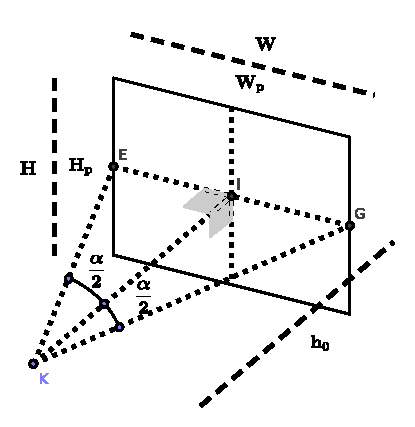
\includegraphics[width=6.0cm]{./images/camera.eps}
\caption{Angulo, $\alpha$, de visão horizontal da câmera.}
\label{fig:camera}
\end{figure} 
A Tabela \ref{tab:tab0} mostra o único parâmetro físico da câmera que será usado
para obter o mapa de disparidade.

\begin{table}[htbp]
\caption{Dados físico-mecânicos da câmera.}
\begin{tcolorbox}[tabgrey,tabularx={c||p{8cm}|Y|},title=Dados da câmera,boxrule=0.5pt]
variável   & Descrição     & Unidades     \\\hline\hline
$\alpha$   & Angulo de visão horizontal da câmera. & radianos \\ \hline
\end{tcolorbox}
\label{tab:tab0}
\end{table}
$W_p$ é $H_p$ são o comprimento e a altura da imagem em pixeis. Estos dados
são extraídos do arquivo de imagem, pelo qual são fáceis de obter.
Se considera que a câmera 1 e a câmera 2 geram arquivos de imagem do mesmo comprimento em pixeis.
A Tabela \ref{tab:tab3} mostra os dados do arquivos de imagem 
que serão usados para obter o mapa de disparidade.
\begin{table}[htbp]
\caption{Dados de comprimento e altura em pixeis provenientes do arquivo da imagem.}
\begin{tcolorbox}[tabgrey,tabularx={c||p{8cm}|Y|},title=Dados dos arquivos,boxrule=0.5pt]
variável  & Descrição     & Unidades     \\\hline\hline
$W_p$   & Largura da imagem. & pixeis \\ \hline
$H_p$   & Altura da imagem. & pixeis \\ \hline
\end{tcolorbox}
\label{tab:tab3}
\end{table}

\subsection{Dados da geometria do problema}

Dado que se terão duas câmeras deslocadas e rotacionadas no espaço, como mostra  
a Figura \ref{fig:modelosimple}, para obter o mapa de disparidade deve-se assumir que
se tem informação do deslocamento e do giro da câmera.
O deslocamento será medido em referencia da câmera 1, assim um deslocamento de $(S_0,S_2,S_1)_{c1}$
indicará que a câmera 2 está localizada a uma distancia $S_0$ à direita da imagem 1, 
a uma distancia $S_2$ para acima da imagem 1,
e a uma distancia $S_1$ no eixo $+Z$ da base canônica da câmera 1.
Por definição se considera que a câmera 1 não tem giro nenhum. 
O giro da câmera 2 é medido em referencia da base canônica da câmera 2, que é paralela à
base canônica da câmera 1. A matriz $M_{N \rightarrow C}$ representa a matriz de transformação de um ponto, $A$,
na base natural da câmera 2 a seu equivalente, $B$, na base canônica da mesma câmera.
\begin{equation}
 B=M_{N \rightarrow C}~A
\end{equation}
A Tabela \ref{tab:tab1} mostra os dados da geometria que serão usados para obter o mapa de disparidade.
\begin{table}[htbp]
\caption{Dados provenientes do analises da geometria do sistema.}
\begin{tcolorbox}[tabgrey,tabularx={X||p{10cm}|Y|},title=Dados da geometria,boxrule=0.5pt]
variável  & Descrição     & Unidades     \\\hline\hline
$S_0$   & Deslocamento da câmera 2 no eixo $+X$ em referencia à câmera 1. & metros \\ \hline
$S_1$   & Deslocamento da câmera 2 no eixo $+Z$ em referencia à câmera 1. & metros \\ \hline
$S_2$   & Deslocamento da câmera 2 no eixo $+Y$ em referencia à câmera 1. & metros \\ \hline
$M_{N \rightarrow C}$  & Matriz de troca de base de um ponto na base natural (em pixeis ou em metros) à base canônica.  & adimensional \\ \hline
\end{tcolorbox}
\label{tab:tab1}
\end{table}


\subsection{Dados do reconhecimento de pontos de coincidência}
Entre  os dados mais importantes para a obtenção do mapa de disparidade, estão
os pontos de coincidência. Estes consistem em pares de pontos $\{D_{1p},D_{2p}\}$,
que representam um ponto $D_{1p}=(x_{1p},y_{1p})$ em pixeis na imagem 1 e seu correspondente, $D_{2p}=(x_{2p},y_{2p})$, 
visto na imagem 2. Lembrando que a imagem 1 e a imagem 2 tem seus eixos coordenado, bidimensionais, referenciados
à base natural das câmeras 1 e 2.
A Tabela \ref{tab:tab2} mostra os dados de pontos de coincidência que serão usados para obter o mapa de disparidade.
\begin{table}[htbp]
\caption{Dados provenientes do reconhecimento de pontos de coincidentes.}
\begin{tcolorbox}[tabgrey,tabularx={c||p{8cm}|Y|},title=Dados de pontos coincidentes,boxrule=0.5pt]
variável  & Descrição     & Unidades     \\\hline\hline
$x_{1p}$   & Distancia no eixo $X$, medida na imagem da câmera 1. & pixeis \\ \hline
$y_{1p}$   & Distancia no eixo $Y$, medida na imagem da câmera 1. & pixeis \\ \hline
$x_{2p}$   & Distancia no eixo $X$, medida na imagem da câmera 2. & pixeis \\ \hline
$y_{2p}$   & Distancia no eixo $Y$, medida na imagem da câmera 2. & pixeis \\ \hline
\end{tcolorbox}
\label{tab:tab2}
\end{table}

\section{Solução do problema}
Para resolver o problema dividiremos este em duas partes. Na primeira tomaremos
em conta só que a imagem está deslocada ( Seção \ref{subsec:desloca}) e não existe giro de câmeras. 
Na segunda só se analisará o giro da câmera 2, 
e se corrigirá o ponto $D_{2p}$ na base natural da câmera 2 para que fique expressado na base canônica
da mesma câmera. Logicamente este novo ponto terá que ser projetado a um plano de imagem virtual na base canônica,
para mais detalhes ver a Seção \ref{subsec:gira}.

\subsection{Câmeras deslocadas} \label{subsec:desloca}
Nesta seção se considera que não existe rotação dos eixos das câmeras, pelo qual a base canônica da câmera 2
será a mesma que sua base natural.
A Figura \ref{fig:dispar} mostra a disposição geométrica de duas câmeras deslocadas no espaço, onde
o ponto $(S_0,S_2,S_1)_{c1}$ representa o deslocamento da câmera 2 em referencia à base canônica da câmera 1.
Também pode-se ver o ponto $P$, que representa o objeto em estudo ao qual deseja-se obter a sua disparidade,
é dizer a sua distancia no eixo $+Z$ referenciado à base canônica das câmeras.
Observa-se que este ponto pode ser representado na base canônica da câmera 1 como $(X_1,Y_1,Z_1)_{c1}$ e na base 
canônica da câmera 2 como $(X_2,Y_2,Z_2)_{c2}$. Pelo Teorema \ref{teo:disparidad1} sabemos que,
\begin{figure}[!]
\center
 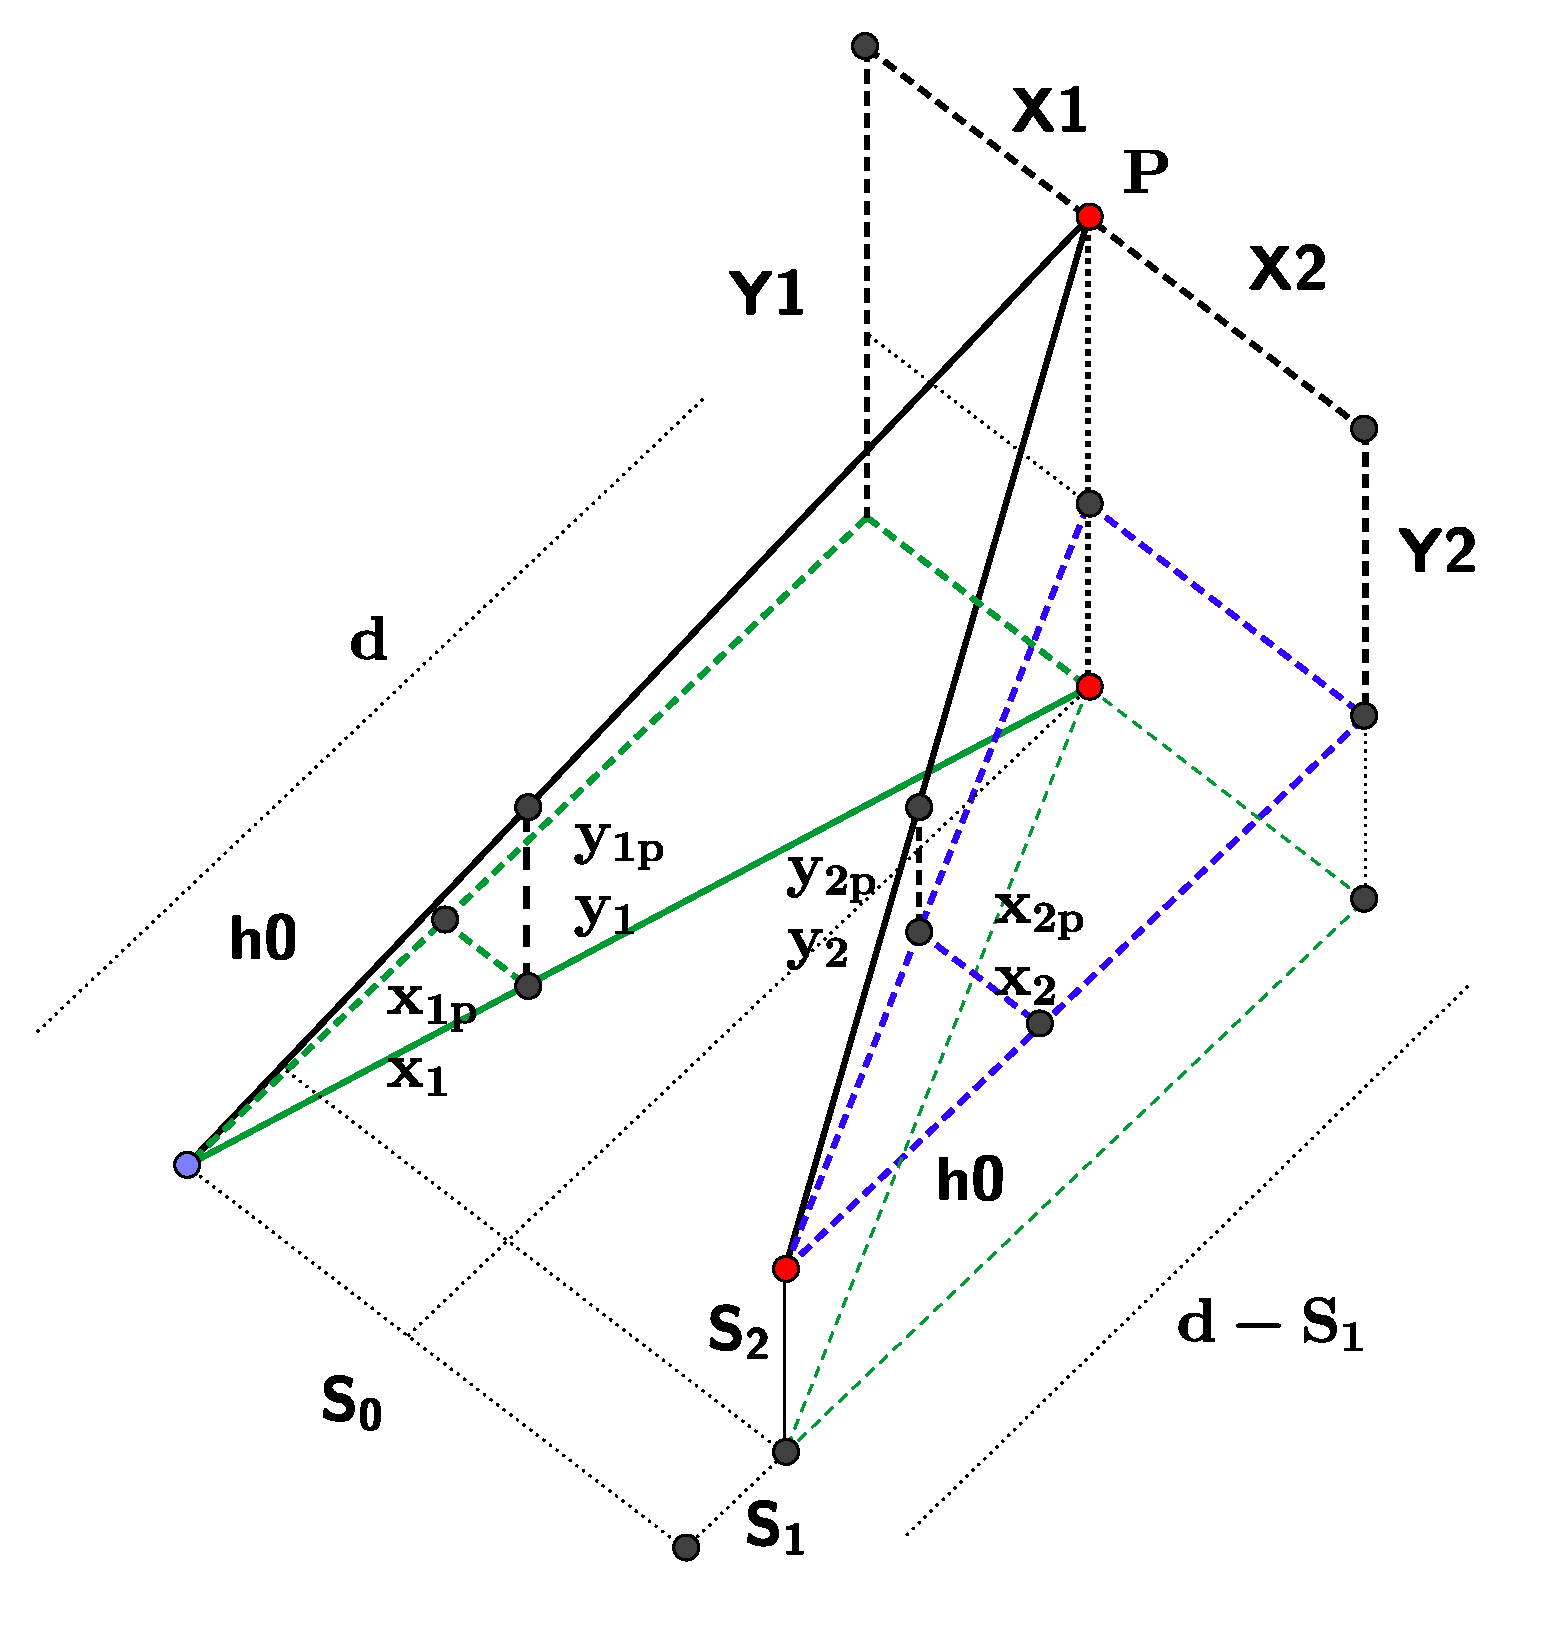
\includegraphics[width=9.0cm]{./images/Diagrama.eps}
\caption{Posição de duas câmeras deslocadas no espaço.}
\label{fig:dispar}
\end{figure} 
\begin{equation}\label{eq:desloca2}
 X_1=2 tan(\frac{\alpha}{2})d\frac{x_{1p}}{W_p},
\end{equation}
\begin{equation}\label{eq:desloca2a}
 Y_1=2 tan(\frac{\alpha}{2})d\frac{y_{1p}}{W_p},
\end{equation}
\begin{equation}\label{eq:desloca4}
 Z_1=d,
\end{equation}
e que,
\begin{equation}\label{eq:desloca3}
 X_2=2 tan(\frac{\alpha}{2})(d-S1)\frac{x_{2p}}{W_p},
\end{equation}
\begin{equation}\label{eq:desloca3a}
 Y_2=2 tan(\frac{\alpha}{2})(d-S1)\frac{y_{2p}}{W_p},
\end{equation}
\begin{equation}\label{eq:desloca4a}
 Z_2=d-S_1.
\end{equation}
Onde $d$ pode ser calculado ate de duas formas distintas. 
Se $x_{1p}\neq x_{2p}$ então
\begin{equation}\label{eq:desloca1}
 d=d_W \equiv \frac{cot(\frac{\alpha}{2})}{2} \frac{W_p S_0}{(x_{1p}-x_{2p})}-\frac{x_{2p} S_1}{(x_{1p}-x_{2p})},
\end{equation}
e se $y_{1p}\neq y_{2p}$ então
\begin{equation}\label{eq:desloca1a}
 d=d_H \equiv \frac{cot(\frac{\alpha}{2})}{2} \frac{W_p S_2}{(y_{1p}-y_{2p})}-\frac{y_{2p} S_1}{(y_{1p}-y_{2p})}.
\end{equation}
Um conjunto valido de pontos $\{D_{1p},D_{2p}\}$, com $x_{1p} \neq x_{2p}$ e $y_{1p} \neq y_{2p}$, sempre cumprirá ambas equações.
De não cumprir-se que $x_{1p} \neq x_{2p}$ ou $y_{1p} \neq y_{2p}$, a sua equação  de cálculo de $d$ se descarta e se usa a outra. 
Na resolução do Teorema \ref{teo:disparidad1}, está explicado que acontece se $x_{1p} = x_{2p}$ e/ou $y_{1p} = y_{2p}$.
~\\

\begin{bclogo}[couleur=gray!30, arrondi=0.1,logo=\bccrayon,ombre=true]{}
Um dado interessante pode ser obtido mediante o Corolário \ref{coro:superficie},
onde sabe-se que se $x_{1p}\neq x_{2p}$ e $y_{1p}\neq y_{2p}$, então um ponto  $\gamma_p=(x_{1p},x_{2p},y_{1p},y_{2p})$
que é  válido (proveniente de um ``match'' certo), cumpre a seguinte equação
 \begin{equation}\label{eq:funccoro1}
  0 = f(x_{1p},x_{2p},y_{1p},y_{2p}) \equiv (K S_2-y_{2p})(x_{1p}-x_{2p})-(K S_0-x_{2p})(y_{1p}-y_{2p})
 \end{equation}
com $K \equiv \frac{cot(\alpha/2)}{2}\frac{W_p}{S_1}$.\\
\end{bclogo}
~\\
\begin{bclogo}[couleur=gray!30, arrondi=0.1,logo=\bccrayon,ombre=true]{}
No caso de tiver um ponto $\hat{\gamma}_p=(\hat{x}_{1p},\hat{x}_{2p},\hat{y}_{1p},\hat{y}_{2p})$ que
não cumpre a equação \ref{eq:funccoro1}, que é equivalente a dizer que $d_H \neq d_W$. Pode-se optar por usar o Corolário \ref{coro:tiko} para achar 
um ponto $\gamma_p$ na superfície de $0=f(\gamma_p)$ que tenha a mínima distancia com $\hat{\gamma}_p$.\\
\end{bclogo}


\subsection{Câmera 2 girada} \label{subsec:gira}
Ate agora tem-se obtido o mapa de disparidade para duas câmaras deslocadas,
quando os eixos canônicos são os mesmos do seus respectivos eixos naturais. 

Nesta seção se analisará o caso quando a câmera 2 tem sua base natural rotacionada em relação a sua base canônica.
Para isto temos que imaginar que depois da obtenção dos pontos de coincidência, ``match'' do ponto $P$,
foram retornados dois pontos, um para imagem 1 e outro para imagem 2. Estes apontam a um mesmo
objeto, ponto $P$, visto de duas perspetivas distintas (câmera 1 e 2). 
É importante lembrar que as imagens retornadas pelas câmeras sempre estão referenciadas a base natural.
Assim, o ponto bidimensional sobre a imagem 2, nesta seção será chamado de $D_{2Np}$, 
onde o sub-índice $2Np$ indica que corresponde a câmera 2,
está referenciado à base natural e usa unidades em pixeis.

Para poder reusar o procedimento desenvolvido na Seção \ref{subsec:desloca} é necessário projetar
o ponto $D_{2Np}$ do plano de imagem na base natural a um plano de imagem, ``virtual'', na base canônica.
Esta projeção será chamada de ponto $D_{2p}$, e também será um ponto bidimensional.
A Figura \ref{fig:cambiodebase} mostra esta distribuição de pontos mais detalhadamente.

Seguindo o Teorema \ref{teo:matcambio} sabe-se que: se a partir de $D_{2Np}=(x_{2Np},y_{2Np})$
criamos o ponto tridimensional
\begin{equation}\label{eq:girac1}
 P_{2Np}=\left(
 \begin{matrix}
  x_{2Np}\\
  y_{2Np}\\
  \frac{cot(\alpha/2)}{2}{W_p}
 \end{matrix}
 \right),
\end{equation}
podemos avaliar a seguinte equação
\begin{equation}\label{eq:girac2}
 D^T_{2p}=\frac{W_p cot(\alpha/2)}{2 }\frac{e_{xy} M_{N \rightarrow C}~P_{2Np} }{ {e_z~M_{N \rightarrow C}~P_{2Np}}},
\end{equation}
para obter o ponto $D_{2p}=(x_{2p},y_{2p})$, onde $e_{xy}$ e $e_z$ são definidos em \eqref{eq:cam8} e \eqref{eq:cam8a}, respectivamente.




\begin{figure}[!]
\center
 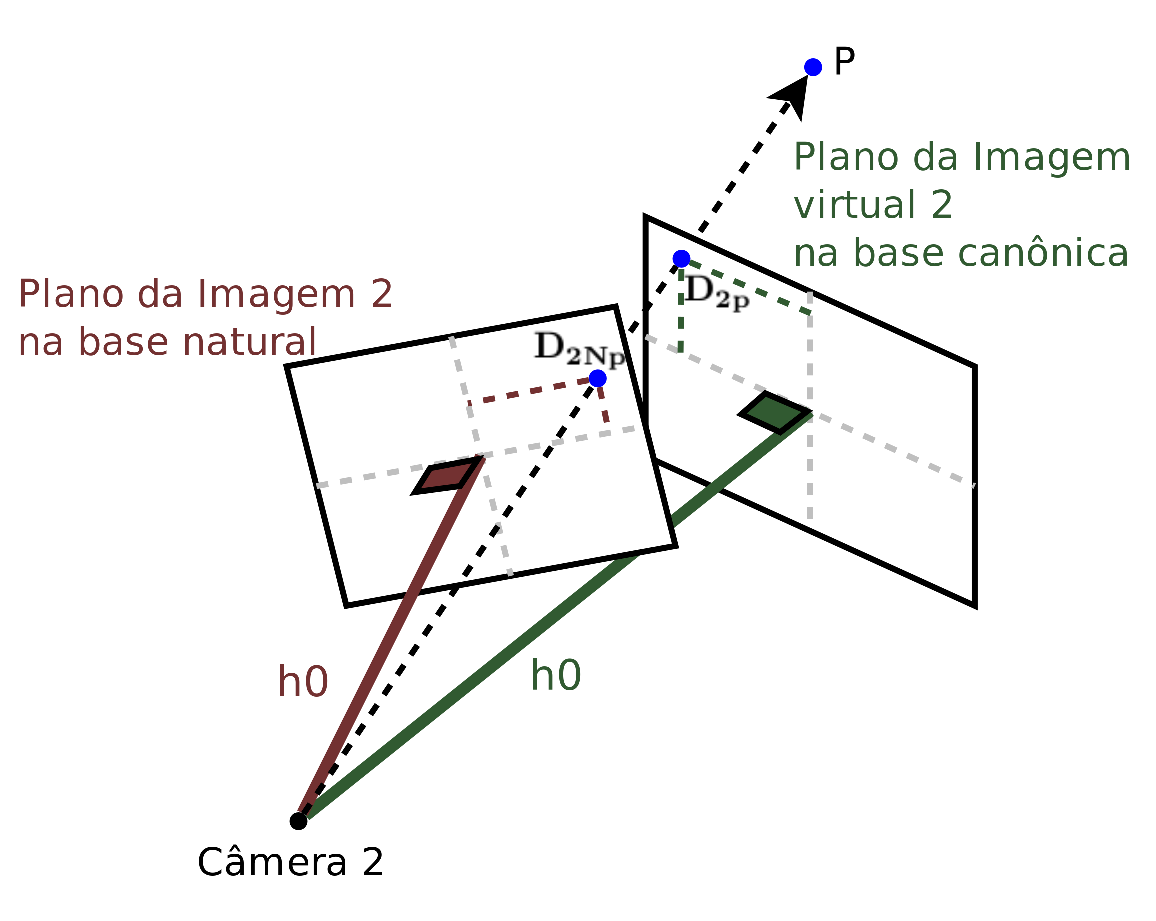
\includegraphics[width=11.0cm]{./images/cambiodebase.eps}
\caption{Plano da imagem na base natural versus o plano da imagem virtual na base canônica.}
\label{fig:cambiodebase}
\end{figure} 

Finalmente o ponto $D_{2p}$ será utilizado para el cálculo del mapa de disparidade
como é explicado na Seção \ref{subsec:desloca}.




\section{Anexo}

%%%%%%%%%%%%%%%%%%%%%%%%%%%%%%%%%%%%%%%%%%%%%%%%%%%%%%%%%%%%%%%%%%%%%%%%%%%%%%%%
%%%%%%%%%%%%%%%%%%%%%%%%%%%%%%%%%%%%%%%%%%%%%%%%%%%%%%%%%%%%%%%%%%%%%%%%%%%%%%%%
\begin{theoremtcolorbox}{Cálculo de disparidade}{disparidad1}
Dadas duas câmeras, câmera 1 e câmera 2 como mostra a Figura \ref{fig:dispar}, que tem
eixos de referencia diferentes mas paralelos e estão separados uma distancia 
$(\bigtriangleup X, \bigtriangleup Y,\bigtriangleup Z)_{c1}=(S_0, S_1, S_2)_{c1}$,
referenciado à câmera 1.
Estas observam um mesmo ponto $P$ seguindo seus respetivos eixos de referencia, 
tendo assim observações $P_{c1}$ e $P_{c2}$ respectivamente.
Pelo qual, seguindo o eixo de referencia da câmera 1, $P_{c1}$ será igual a:
\begin{equation}\label{eq:Pc1}
P_{c1}=(X_1,Y_1,Z_1)_{c1}
\end{equation}
e seguindo o eixo de referencia da câmera 2, $P_{c2}$ será igual a:
\begin{equation}\label{eq:Pc2}
P_{c2}=(X_2,Y_2,Z_2)_{c2}.
\end{equation}
Onde
\begin{equation}\label{eq:res2}
 X_1=2 tan(\frac{\alpha}{2})d\frac{x_{1p}}{W_p}~\wedge~Y_1=2 tan(\frac{\alpha}{2})d\frac{y_{1p}}{W_p}
\end{equation}
\begin{equation}\label{eq:res3}
 X_2=2 tan(\frac{\alpha}{2})(d-S1)\frac{x_{2p}}{W_p}~\wedge~Y_2=2 tan(\frac{\alpha}{2})(d-S1)\frac{y_{2p}}{W_p}
\end{equation}
\begin{equation}\label{eq:res4}
 ~~~~~~~~Z_1=d~\wedge~Z_2=d-S_1.
\end{equation}
Sendo que se $x_{1p}\neq x_{2p}$ então
\begin{equation}\label{eq:res1}
 d=d_W \equiv \frac{cot(\frac{\alpha}{2})}{2} \frac{W_p S_0}{(x_{1p}-x_{2p})}-\frac{x_{2p} S_1}{(x_{1p}-x_{2p})}
\end{equation}
e/ou se $y_{1p}\neq y_{2p}$ então
\begin{equation}\label{eq:res1a}
 d= d_H \equiv \frac{cot(\frac{\alpha}{2})}{2} \frac{W_p S_2}{(y_{1p}-y_{2p})}-\frac{y_{2p} S_1}{(y_{1p}-y_{2p})}.
\end{equation}
\end{theoremtcolorbox}
%%%%%%%%%%%%%%%%%%%%%%%%%%%%%%%%%%%%%%%%%%%%%%%%%%%%%%%%%%%%%%%%%%%%%%%%%%%%%%%%
\begin{proof}
O primeiro que podemos assumir, é que a proporção relativa entre a largura e a altura da imagem,
é a mesma em metros que em pixeis.
\begin{equation}\label{eq:sup1}
\frac{W}{H}=\frac{W_p}{H_p}
\end{equation}
Isto é natural porque de não cumprir-se existiria uma distorção na imagem em pixeis ao ser representada de forma visual.
A proporcionalidade definida na equação \eqref{eq:sup1} leva a afirmar para o ponto $(x_{1},y_{1})$ que
\begin{equation}\label{eq:sup2}
\frac{x_1}{x_{1p}}=\frac{W}{W_p}
\end{equation}
\begin{equation}\label{eq:sup2a}
\frac{y_1}{y_{1p}}=\frac{H}{H_p},
\end{equation}
e similarmente para o ponto $(x_{2},y_{2})$ que
\begin{equation}\label{eq:sup3}
\frac{x_2}{x_{2p}}=\frac{W}{W_p}
\end{equation}
\begin{equation}\label{eq:sup3a}
\frac{y_2}{y_{2p}}=\frac{H}{H_p}.
\end{equation}
Usando a Figura \ref{fig:dispar} e o Teorema \ref{teo:propor}
pode-se afirmar que 
\begin{equation}\label{eq:sup4}
\frac{X_1}{x_{1}}=\frac{d}{h_0}~\wedge~\frac{X_2}{x_{2}}=\frac{d-S_1}{h_0}
\end{equation}
e
\begin{equation}\label{eq:sup5}
\frac{Y_1}{y_{1}}=\frac{d}{h_0}~\wedge~\frac{Y_2}{y_{2}}=\frac{d-S_1}{h_0}
\end{equation}
Pela geometria do problema também pode-se afirmar que 
\begin{equation}\label{eq:sup6}
X_1-X_2=S_0,
\end{equation}
\begin{equation}\label{eq:sup7}
Y_1-Y_2=S_2.
\end{equation}
Agora, incluindo a equações \eqref{eq:sup2}, e \eqref{eq:sup3} em \eqref{eq:sup4}
obtemos
\begin{equation}\label{eq:sup4a}
X_1=d\frac{x_{1p}}{W_p}\frac{W}{h_0}~\wedge~X_2=(d-S_1)\frac{x_{2p}}{W_p}\frac{W}{h_0},
\end{equation}
e incluindo a equações \eqref{eq:sup2a}, e \eqref{eq:sup3a} em \eqref{eq:sup5}
obtemos
\begin{equation}\label{eq:sup5a}
Y_1=d\frac{y_{1p}}{H_p}\frac{H}{h_0}~\wedge~Y_2=(d-S_1)\frac{y_{2p}}{H_p}\frac{H}{h_0}.
\end{equation}

\textbf{Caso quando $\mathbf{x_{1p}\neq x_{2p}}$:}\\
Assim, se assumimos que $x_{1p}\neq x_{2p}$ e incluímos a equação \eqref{eq:sup4a} em \eqref{eq:sup6} obtemos que
\begin{equation}\label{eq:sup6b}
 \frac{d}{W_p}\frac{W}{h_0} (x_{1p}-x_{2p})=  S_0- S_1 \frac{x_{2p}}{W_p}\frac{W}{h_0}
\end{equation}
e 
\begin{equation}\label{eq:sup6a}
 d=\frac{h_0}{W} \frac{W_p S_0}{(x_{1p}-x_{2p})}-\frac{x_{2p} S_1}{(x_{1p}-x_{2p})}.
\end{equation}

\textbf{Caso quando $\mathbf{x_{1p}= x_{2p}}=x_{p}$:}\\
No caso contrario, se assumimos que $x_{1p}= x_{2p}=x_p$ e incluímos a equação \eqref{eq:sup4a} 
em \eqref{eq:sup6} obtemos a seguinte restrição para $x_p$
\begin{equation}\label{eq:sup6c}
 S_0 = S_1 \frac{x_{p}}{W_p}\frac{W}{h_0},
\end{equation}
e nenhuma para a variável $d$.

\textbf{Caso quando $\mathbf{y_{1p}\neq y_{2p}}$:}\\
Por outro lado se assumimos que $y_{1p}\neq y_{2p}$ e incluímos  a equação \eqref{eq:sup5a} em \eqref{eq:sup7} obtemos que
\begin{equation}\label{eq:sup7b}
 \frac{d}{H_p}\frac{H}{h_0} (y_{1p}-y_{2p})=  S_2- S_1 \frac{y_{2p}}{H_p}\frac{H}{h_0}
\end{equation}
e 
\begin{equation}\label{eq:sup7a}
 d=\frac{h_0}{H} \frac{H_p S_2}{(y_{1p}-y_{2p})}-\frac{y_{2p} S_1}{(y_{1p}-y_{2p})}.
\end{equation}

\textbf{Caso quando $\mathbf{y_{1p}= y_{2p}}=y_{p}$:}\\
No caso contrario, se assumimos que $y_{1p}= y_{2p}=y_p$ e incluímos a equação \eqref{eq:sup5a} 
em \eqref{eq:sup7} obtemos a seguinte restrição para $y_p$
\begin{equation}\label{eq:sup7c}
 S_2 = S_1 \frac{y_{p}}{H_p}\frac{H}{h_0},
\end{equation}
e nenhuma para a variável $d$.\\

É fácil de ver que o único caso onde $x_{1p}= x_{2p}$ e $y_{1p}= y_{2p}$ será quando
as duas câmeras estejam na mesma posição e com suas bases naturais em eixos paralelos.
Para os demais casos, pelo menos uma de estas igualdades não será cumprida, e variavel
$d$ poderá ser calculada.

Agora, tendo o valor da variável $d$ em \eqref{eq:sup6a} e/ou \eqref{eq:sup7a}, 
e usando o Teorema \ref{teo:angulo}
para substituir ${h_0}/{W}$ e ${h_0}/{H}$, pode-se afirmar que as
equações \eqref{eq:res1} e \eqref{eq:res1a} são verdadeiras. 
Da mesma forma pode ser substituído o valor  ${h_0}/{W}$ e ${h_0}/{H}$ nas
equações \eqref{eq:sup4a} e \eqref{eq:sup5a}, obtendo-se as equações
\eqref{eq:res2} e \eqref{eq:res3}.
\end{proof}


%%%%%%%%%%%%%%%%%%%%%%%%%%%%%%%%%%%%%%%%%%%%%%%%%%%%%%%%%%%%%%%%%%%%%%%%%%%%%%%%
%%%%%%%%%%%%%%%%%%%%%%%%%%%%%%%%%%%%%%%%%%%%%%%%%%%%%%%%%%%%%%%%%%%%%%%%%%%%%%%%
\begin{corollarytcolorbox}{Superfície 4-dimensional de pontos válidos }{superficie}
 Seguindo o Teorema \ref{teo:disparidad1}, sobre um sistema onde as bases naturais das câmeras
 são paralelas entre sim, como na Figura \ref{fig:dispar}, sabe-se que se os pontos $D_{1p}=(x_{1p},y_{1p})$ e
 $D_{2p}=(x_{2p},y_{2p})$ cumprem que $x_{1p}\neq x_{2p}$ e $y_{1p}\neq y_{2p}$, então eles pertencem à superfície
 \begin{equation}\label{eq:func1}
 0=f(x_{1p},x_{2p},y_{1p},y_{2p})\equiv f(\gamma_p),
 \end{equation}
onde
 \begin{equation}\label{eq:func2}
  f(x_{1p},x_{2p},y_{1p},y_{2p}) \equiv (KS_2-y_{2p})(x_{1p}-x_{2p})-(KS_0-x_{2p})(y_{1p}-y_{2p})
 \end{equation}
 e
 \begin{equation}\label{eq:func3}
  K \equiv \frac{cot(\frac{\alpha}{2})}{2}\frac{W_p}{S_1}
 \end{equation} 
\end{corollarytcolorbox}
%%%%%%%%%%%%%%%%%%%%%%%%%%%%%%%%%%%%%%%%%%%%%%%%%%%%%%%%%%%%%%%%%%%%%%%%%%%%%%%%
\begin{proof}
 Igualando as equações \eqref{eq:res1} e \eqref{eq:res1a}
 \begin{equation}\label{eq:func4}
 \frac{W_p cot(\frac{\alpha}{2})}{2} \left (\frac{ S_2}{(y_{1p}-y_{2p})} - \frac{ S_0}{(x_{1p}-x_{2p})}\right ) = S_1 \left (\frac{y_{2p} }{(y_{1p}-y_{2p})} - \frac{x_{2p} }{(x_{1p}-x_{2p})} \right ).
\end{equation}
Usando a definição \eqref{eq:func3} obtemos
 \begin{equation}\label{eq:func4a}
 K \left (\frac{ S_2}{(y_{1p}-y_{2p})} - \frac{ S_0}{(x_{1p}-x_{2p})}\right ) =  \left (\frac{y_{2p} }{(y_{1p}-y_{2p})} - \frac{x_{2p} }{(x_{1p}-x_{2p})} \right ).
\end{equation}
Reordenando a equação anterior, temos
\begin{equation}\label{eq:func5}
 K \left ({ S_2}{(x_{1p}-x_{2p})} - { S_0}{(y_{1p}-y_{2p})}\right ) =  \left ({y_{2p} }{(x_{1p}-x_{2p})} - {x_{2p} }{(y_{1p}-y_{2p})} \right ),
\end{equation}
e finalmente
\begin{equation}\label{eq:func6}
 (K { S_2}-y_{2p}){(x_{1p}-x_{2p})} - (K{ S_0}-x_{2p}){(y_{1p}-y_{2p})} =   0.
\end{equation}
\end{proof}

%%%%%%%%%%%%%%%%%%%%%%%%%%%%%%%%%%%%%%%%%%%%%%%%%%%%%%%%%%%%%%%%%%%%%%%%%%%%%%%%
%%%%%%%%%%%%%%%%%%%%%%%%%%%%%%%%%%%%%%%%%%%%%%%%%%%%%%%%%%%%%%%%%%%%%%%%%%%%%%%%
\begin{corollarytcolorbox}{Ponto na superfície $0=f(\gamma_p)$ com a menor distancia a $\hat{\gamma}_p$}{tiko}
 Seguindo o Teorema \ref{teo:disparidad1} e o Corolário \ref{coro:superficie}, 
 sobre um sistema onde as bases naturais das câmeras
 são paralelas entre sim, como na Figura \ref{fig:dispar}. 
 Sim se tem um ponto $\hat{\gamma}_p=(\hat{x}_{1p},\hat{x}_{2p},\hat{y}_{1p},\hat{y}_{2p})$ 
 que não pertence  à superfície $0=f(\gamma_p)\equiv (KS_2-y_{2p})(x_{1p}-x_{2p})-(KS_0-x_{2p})(y_{1p}-y_{2p})$
 com $K=\frac{cot(\frac{\alpha}{2})}{2}\frac{W_p}{S_1}$. 
 
 Então o ponto  $\gamma_p$ mais próximo a $\hat{\gamma}_p$ na superfície  $0=f(\gamma_p)$, pode ser achado
 com a seguinte equação iterativa de $\beta=(x_{1p},x_{2p},y_{1p},y_{2p},\lambda)^T$.
 \begin{equation}\label{eq:t1}
 \beta_{i+1} := \beta_{i} - \left [ \mathbf{J}^T(\beta_i) \mathbf{J}(\beta_i) \right ]^{-1} \mathbf{J}^T(\beta_i) \mathbf{G}(\beta_i),
 \end{equation}
 onde 
\begin{equation}\label{eq:t3}
 \mathbf{G}(\beta)=\left(
 \begin{matrix}
 2(x_{1p}-\hat{x}_{1p})+ \lambda (K S_2 -y_{2p})\\
 2(x_{2p}-\hat{x}_{2p})+ \lambda ( y_{1p} - K S_2)\\
 2(y_{1p}-\hat{y}_{1p})+ \lambda (x_{2p} - K S_0)\\
 2(y_{2p}-\hat{y}_{2p})+ \lambda ( K S_0 - x_{1p})\\
 (KS_2-y_{2p})(x_{1p}-x_{2p})-(KS_0-x_{2p})(y_{1p}-y_{2p})
 \end{matrix} 
 \right)
\end{equation} 
 
\begin{equation}\label{eq:t4}
 \mathbf{J}(\beta)=\left(
 \begin{matrix}
  2&0&0&-\lambda&(K S_2 - y_{2p})\\
  0&2&\lambda&0&(y_{1p}-K S_2)\\
  0&\lambda&2&0&(x_{2p}-K S_0)\\
  -\lambda&0&0&2&(K S_0 -x_{1p}\\
  (K S_2 - y_{2p})&(y_{1p}-K S_2)&(x_{2p}-K S_0)&(K S_0-x_{1p})&0
 \end{matrix}
 \right),
\end{equation}
é sugerido que o valor inicial de $\beta_0$  seja 
\begin{equation}\label{eq:t2}
 \beta_{0}=\left(
 \begin{matrix}
 \hat{x}_{1p}\\
 \hat{x}_{2p}\\
 \hat{y}_{1p}\\
 \hat{y}_{2p}\\
 0
 \end{matrix}
 \right),
 \end{equation}
 dado que considera-se que o ponto $(\hat{x}_{1p}, \hat{x}_{2p}, \hat{y}_{1p}, \hat{y}_{2p})$
 já está próximo à superfície. \\
 
 \textbf{Nota:} Deve-se tomar cuidado que os valores iniciais e as soluções
 cumpram que $x_{1p} \neq x_{2p}$ e $y_{1p} \neq y_{2p}$. De não cumprir-se alguma destas equações,
 deve-se tomar em conta as equações \eqref{eq:sup6c} e \eqref{eq:sup7c}, e agregar valores aleatórios ao vetor $\gamma_p$ para evitar cair em mínimos locais.
\end{corollarytcolorbox}
%%%%%%%%%%%%%%%%%%%%%%%%%%%%%%%%%%%%%%%%%%%%%%%%%%%%%%%%%%%%%%%%%%%%%%%%%%%%%%%%
\begin{proof}

Para obter o ponto $\gamma_p$ 
com a distancia mínima, do ponto $\hat{\gamma}_p$ à superfície $0=f(\gamma_p)$,
usa-se a formulação de Lagrange, 
\begin{equation}\label{eq:tikon1a}
 L(\gamma_p,\lambda)= ||\gamma_p-\hat{\gamma}_p||^2+\lambda f(\gamma_p),
\end{equation}
\begin{equation}\label{eq:tikon1}
 L(\gamma_p,\lambda)=(x_{1p}-\hat{x}_{1p})^2+(x_{2p}-\hat{x}_{2p})^2+(y_{1p}-\hat{y}_{1p})^2+(y_{2p}-\hat{y}_{2p})^2 +\lambda f(x_{1p},x_{2p},y_{1p},y_{2p})
\end{equation}
de modo que
\begin{equation}\label{eq:tikon2}
 \frac{\partial L(\gamma_p,\lambda)}{\partial x_{1p}}=2(x_{1p}-\hat{x}_{1p})+ \lambda (K S_2 -y_{2p})=0 
\end{equation}
\begin{equation}\label{eq:tikon3}
 \frac{\partial L(\gamma_p,\lambda)}{\partial x_{2p}}=2(x_{2p}-\hat{x}_{2p})+ \lambda ( y_{1p} - K S_2)=0 
\end{equation}
\begin{equation}\label{eq:tikon4}
 \frac{\partial L(\gamma_p,\lambda)}{\partial y_{1p}}=2(y_{1p}-\hat{y}_{1p})+ \lambda (x_{2p} - K S_0)=0 
\end{equation} 
\begin{equation}\label{eq:tikon5}
 \frac{\partial L(\gamma_p,\lambda)}{\partial y_{2p}}=2(y_{2p}-\hat{y}_{2p})+ \lambda ( K S_0 - x_{1p})=0 
\end{equation} 
\begin{equation}\label{eq:tikon6}
 \frac{\partial L(\gamma_p,\lambda)}{\partial \lambda}=(KS_2-y_{2p})(x_{1p}-x_{2p})-(KS_0-x_{2p})(y_{1p}-y_{2p})=0 
\end{equation} 

As equações anteriores podem ser reordenadas como uma função vetorial $\mathbf{G}(\beta)~:~{\Re}^5\rightarrow {\Re}^5$,
com vetor de entrada $\beta=(x_{1p},x_{2p},y_{1p},y_{2p},\lambda)$,
\begin{equation}\label{eq:tikon7}
 0 = \left(
  \frac{\partial L(\beta)}{\partial x_{1p}},
  \frac{\partial L(\beta)}{\partial x_{2p}},
  \frac{\partial L(\beta)}{\partial y_{1p}},
  \frac{\partial L(\beta)}{\partial y_{2p}},
  \frac{\partial L(\beta)}{\partial \lambda},  
 \right)
 =\nabla L(\gamma_p,\lambda) \equiv \mathbf{G}^T(\beta)
\end{equation}
Para achar o vetor $\beta$ que cumpre a equação anterior, usaremos a regularização de Tikhonov
 \cite{shobha2014newton,doicu2002iteratively,tichonov1992ill}. Esta regularização resolve o problema 
 anterior como  a tentativa de achar o valor de $\beta$ que minimiza $e^2$ em
\begin{equation}\label{eq:tikon8}
 e^2= ||\mathbf{G}(\beta)||^2,
\end{equation}
sendo a solução de Tikhonov a seguinte equação iterativa.
\begin{equation}\label{eq:tikon9}
 \beta_{i+1} := \beta_{i} - \left [ \mathbf{J}^T(\beta_i) \mathbf{J}(\beta_i) \right ]^{-1} \mathbf{J}^T(\beta_i) \mathbf{G}(\beta_i)
\end{equation} 
com $\mathbf{J}(\beta)$ igual ao Jacobiano de $\mathbf{G}(\beta)$,
\begin{equation}\label{eq:tikon10}
 \mathbf{J}(\beta)\equiv \frac{\partial \mathbf{G}(\beta)}{\partial \beta}=\left(
 \begin{matrix}
  2&0&0&-\lambda&(K S_2 - y_{2p})\\
  0&2&\lambda&0&(y_{1p}-K S_2)\\
  0&\lambda&2&0&(x_{2p}-K S_0)\\
  -\lambda&0&0&2&(K S_0 -x_{1p}\\
  (K S_2 - y_{2p})&(y_{1p}-K S_2)&(x_{2p}-K S_0)&(K S_0-x_{1p})&0
 \end{matrix}
 \right)
\end{equation}
\end{proof}

%%%%%%%%%%%%%%%%%%%%%%%%%%%%%%%%%%%%%%%%%%%%%%%%%%%%%%%%%%%%%%%%%%%%%%%%%%%%%%%%
%%%%%%%%%%%%%%%%%%%%%%%%%%%%%%%%%%%%%%%%%%%%%%%%%%%%%%%%%%%%%%%%%%%%%%%%%%%%%%%%
\begin{theoremtcolorbox}{Equivalência do angulo $\alpha$}{angulo}
 Dada uma câmera com um angulo de visão horizontal $\alpha$ como mostra a Figura
 \ref{fig:camera}, então é verdade que
\begin{equation} \label{eq:angle1}
 \frac{W}{h_0} =2~tan(\frac{\alpha}{2})
\end{equation}
\begin{equation} \label{eq:angle2}
 \frac{H}{h_0} =2~tan(\frac{\alpha}{2}) \frac{H_p}{W_p}
\end{equation}
\begin{equation} \label{eq:angle3}
 h_{0p} =W_p \frac{cot(\frac{\alpha}{2})}{2}
\end{equation}
\end{theoremtcolorbox}
%%%%%%%%%%%%%%%%%%%%%%%%%%%%%%%%%%%%%%%%%%%%%%%%%%%%%%%%%%%%%%%%%%%%%%%%%%%%%%%%
\begin{proof}
 Na Figura \ref{fig:camera} no triangulo retângulo $EIK$ formado
 pelo ponto médio de $\overline{EG}$ e os ponto $E$ e $K$, pode-se deduzir que
\begin{equation} \label{eq:cam1}
 \frac{W/2}{h_0}=tan(\frac{\alpha}{2}).
\end{equation}
Reordenando a anterior equação obtemos \eqref{eq:angle1}.
Por outro lado é evidente que existe uma proporção comum entre a distancia
em pixeis e em metros. De modo que
\begin{equation} \label{eq:cam3}
 \frac{W}{W_p}=\frac{H}{H_p}=\frac{h_0}{h_{0p}}.
\end{equation}
Usando esta equação em \eqref{eq:cam1} obtemos as equações \eqref{eq:angle2} e \eqref{eq:angle3}.
\end{proof}

%%%%%%%%%%%%%%%%%%%%%%%%%%%%%%%%%%%%%%%%%%%%%%%%%%%%%%%%%%%%%%%%%%%%%%%%%%%%%%%%
%%%%%%%%%%%%%%%%%%%%%%%%%%%%%%%%%%%%%%%%%%%%%%%%%%%%%%%%%%%%%%%%%%%%%%%%%%%%%%%%
\begin{theoremtcolorbox}{Proporcionalidade entre lados}{propor}
Conhecidos dois triângulos $AFE$ e $FIE$ (ver Figura \ref{fig:model}), que são cortados
por as linhas $\overline{HG}=b_1$ e $\overline{GJ}=c_1$ paralelas a $\overline{AF}=b_2$ 
e $\overline{FI}=c_2$ respetivamente, se cumpre a seguinte relação com $\overline{AE}=a_2$ 
e $\overline{HE}=a_1$:
\begin{equation}\label{eq:a0}
 \frac{a_2}{a_1}=\frac{b_2}{b_1}=\frac{c_2}{c_1}
\end{equation}
\end{theoremtcolorbox}
\begin{figure}[!t]
\center
 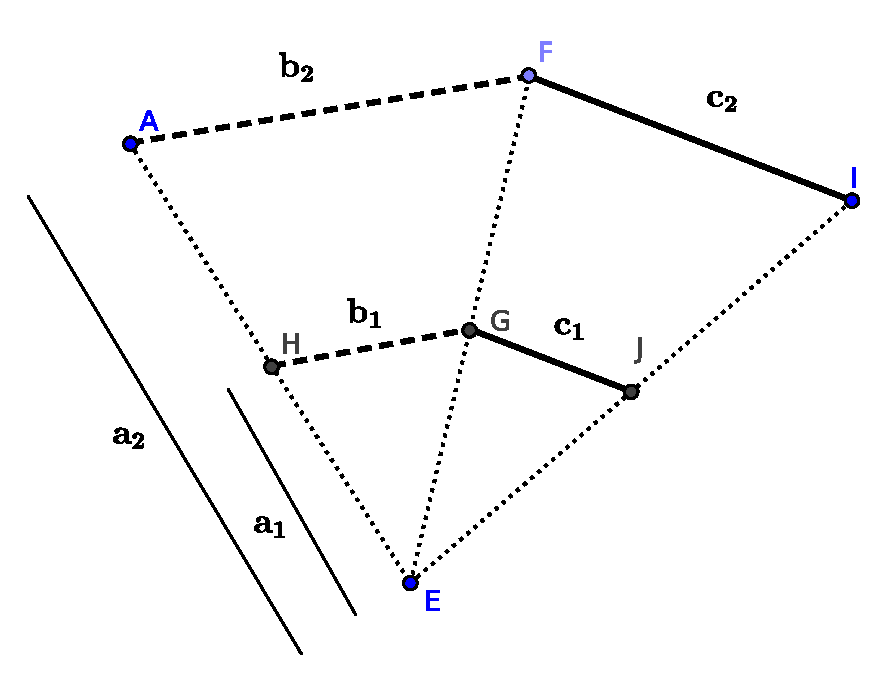
\includegraphics[width=8.0cm]{./images/paralelas.eps}
\caption{Regra das proporções em linhas paralelas.}
\label{fig:model}
\end{figure} 
%%%%%%%%%%%%%%%%%%%%%%%%%%%%%%%%%%%%%%%%%%%%%%%%%%%%%%%%%%%%%%%%%%%%%%%%%%%%%%%%
\begin{proof}
Devido a que os triângulos são cortados por linhas paralelas, podemos afirmar que
o triangulo $HGE$ e o triangulo $AFE$ são semelhantes. Da mesmo forma pode-se afirmar 
que o triangulo $GJE$ é semelhante ao triângulo $FIE$. Pelo qual 
existirá uma proporcionalidade entre seus lados, de modo que
\begin{equation}\label{eq:a1}
 \frac{\overline{AF}}{\overline{HG}}=\frac{\overline{AE}}{\overline{HE}}~~~\wedge~~~ \frac{\overline{FI}}{\overline{GJ}}=\frac{\overline{FE}}{\overline{GE}}.
\end{equation}
Pelo teorema de Tales sobre o triangulo $AFE$, sabemos que
\begin{equation}\label{eq:a2}
 \frac{\overline{AE}}{\overline{HE}}=\frac{\overline{FE}}{\overline{GE}}.
\end{equation}
Das equações \eqref{eq:a1} e \eqref{eq:a2} pode-se deduzir que
\begin{equation}\label{eq:a3}
 \frac{\overline{AE}}{\overline{HE}}=\frac{\overline{AF}}{\overline{HG}}=\frac{\overline{FI}}{\overline{GJ}}.
\end{equation}
e consequentemente a equação \eqref{eq:a0} é verdadeira.
\end{proof}

%%%%%%%%%%%%%%%%%%%%%%%%%%%%%%%%%%%%%%%%%%%%%%%%%%%%%%%%%%%%%%%%%%%%%%%%%%%%%%%%
%%%%%%%%%%%%%%%%%%%%%%%%%%%%%%%%%%%%%%%%%%%%%%%%%%%%%%%%%%%%%%%%%%%%%%%%%%%%%%%%
\begin{theoremtcolorbox}{Método para achar o ponto de coincidência $D_{2p}$ no plano de imagem virtual 2 na base canônica}{matcambio}
Nosso objetivo aqui será trasladar a informação proveniente de um ponto 
$D_{2Np}=(x_{2Np},y_{2Np})$, 
no plano de imagem na base natural da câmera 2 a seu correspondente ponto 
$D_{2p}=(x_{2p},y_{2p})$ na imagem virtual na base canônica, como mostra a Figura \ref{fig:cambiodebase}.

Para isto, definimos as seguintes variáveis
\begin{equation}\label{eq:cam8}
 e_{xy} \equiv \left(
 \begin{matrix}
  1&0&0\\
  0&1&0\\
 \end{matrix}
 \right),
\end{equation}
\begin{equation}\label{eq:cam8a}
 e_{z} \equiv \left(  \begin{matrix}
  0&0&1
 \end{matrix} \right).
\end{equation}
De modo que para obter o ponto $D_{2p}=(x_{2p},y_{2p})$, avaliaremos as equações \eqref{eq:cam7b}, \eqref{eq:cam7a} e \eqref{eq:camp9},
usando como entrada de dados o ponto $D_{2Np}=(x_{2Np},y_{2Np})$ e a matriz de troca de base $M_{N \rightarrow C}$.
\begin{equation}\label{eq:cam7b}
 P_{2Np}=\left(
 \begin{matrix}
  x_{2Np}\\
  y_{2Np}\\
  \frac{cot(\alpha/2)}{2}{W_p}
 \end{matrix}
 \right),
\end{equation}
\begin{equation}\label{eq:cam7a}
 \mu = \frac{2 tan(\alpha/2)}{{W_p}} {e_z~M_{N \rightarrow C}~P_{2Np}},
\end{equation}
\begin{equation}\label{eq:camp9}
 D^T_{2p}=\frac{e_{xy} M_{N \rightarrow C}~P_{2Np} }{\mu}.
\end{equation}
\end{theoremtcolorbox}
%%%%%%%%%%%%%%%%%%%%%%%%%%%%%%%%%%%%%%%%%%%%%%%%%%%%%%%%%%%%%%%%%%%%%%%%%%%%%%%%
\begin{proof}
Primeiro redefinimos o ponto bidimensional, $D_{2Np}$, como um ponto tridimensional
\begin{equation}\label{eq:cam1b}
 P_{2Np}=(x_{2Np},y_{2Np},h_{0p})^T_{2Np},
\end{equation}
localizado a uma distancia $h_{0p}$ (em pixeis) no eixo $+Z$
na base natural da câmera 2. Seu correspondente equivalente
\begin{equation}\label{eq:cam1a}
 P_{2Cp}=(x_{2Cp},y_{2Cp},h_{zp})^T_{2Cp},
\end{equation}
na base canônica, pode ser achado usando a matriz de 
troca de base, $M_{N \rightarrow C}$, que leva um ponto da base natural à base canônica.
Como mostra a seguinte equação
\begin{equation}\label{eq:cam2}
 P_{2Cp} =M_{N \rightarrow C}~P_{2Np}.
\end{equation}
A Figura \ref{fig:model2} mostra esta distribuição de pontos.
Um método para achar a matriz de troca de base pode ser visto em \cite{cambiobase}.

\begin{figure}[!]
\center
 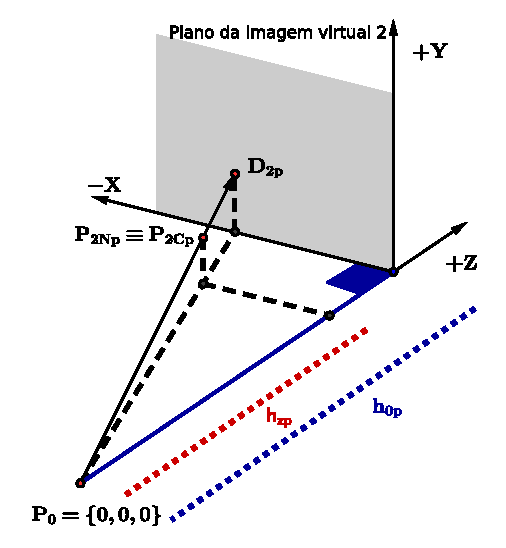
\includegraphics[width=9.0cm]{./images/projetadndo.eps}
\caption{Projeção $D_{2p}$ no plano da imagem virtual na base canônica da câmera 2, proveniente de um ponto $P_{2Cp}$.}
\label{fig:model2}
\end{figure} 

Se redefinimos o ponto bidimensional, $D_{2p}$,  como o ponto tridimensional 
\begin{equation}\label{eq:cam3a}
 P_{2p}=(x_{2p},y_{2p},h_{0p})^T_{2Cp},
\end{equation}
localizado a uma distancia $h_{0p}$ (em pixeis) no eixo $+Z$ da base canônica,
é fácil de ver que $P_{2Cp}$ é proporcional a $P_{2p}$
\begin{equation}\label{eq:cam4}
 P_{2p}= \frac{P_{2Cp}}{\mu} 
\end{equation}
Usando O Teorema \ref{teo:propor} sabe-se que
\begin{equation}\label{eq:cam5}
 \mu = \frac{h_{zp}}{h_{0p}},
\end{equation}
e usando o resultado do Teorema \ref{teo:angulo}
\begin{equation}\label{eq:cam6a}
{h_{0p}} = \frac{cot(\alpha/2)}{2}{W_p},
\end{equation}
de modo que
\begin{equation}\label{eq:cam6}
 \mu = \frac{2 tan(\alpha/2)}{{W_p}}{h_{zp}},
\end{equation}
Se  introduzimos a equação \eqref{eq:cam2} e a definição \eqref{eq:cam8a} na equação anterior obtemos
\begin{equation}\label{eq:cam7}
 \mu = \frac{2 tan(\alpha/2)}{{W_p}} {e_z~M_{N \rightarrow C}~P_{2Np}}.
\end{equation}
Finalmente usando a definição da equação \eqref{eq:cam8} temos que
\begin{equation}\label{eq:camp}
 D^T_{2p}=e_{xy}P_{2p}
\end{equation}
\end{proof}


%%%%%%%%%%%%%%%%%%%%%%%%%%%%%%%%%%%%%%%%%%%%%%%%%%%%%%%%%%%%%%%%%%%%%%%%%%%%%%%%
%%%%%%%%%%%%%%%%%%%%%%%%%%%%%%%%%%%%%%%%%%%%%%%%%%%%%%%%%%%%%%%%%%%%%%%%%%%%%%%%
\begin{theoremtcolorbox}{Analises de erro no cálculo da disparidade quando temos erros no reconhecimento nos pontos de coincidência }{errodisp}
Se consideramos que só o ponto $D_{2p}=(x_{2p},y_{2p})$ está sujeito a erro, dado que 
o ponto $D_{1p}=(x_{1p},y_{1p})$ é escolhido e o ponto $D_{2p}$ é reconhecido. Então
\begin{equation}\label{eq:errodisp2}
 \partial d_W \equiv \frac{h_{0p}S_0-x_{1p}S_1}{(x_{1p}-x_{2p})^2}~\partial x_{2p}
\end{equation}
\begin{equation}\label{eq:errodisp3}
 \partial d_H \equiv \frac{h_{0p}S_2-y_{1p}S_1}{(y_{1p}-y_{2p})^2}~\partial y_{2p}
\end{equation}

De ambas é fácil de ver que o erro cresce assintoticamente quando $x_{1p}-x_{2p}$ ou $y_{1p}-y_{2p}$ tendem a zero.
\end{theoremtcolorbox}
%%%%%%%%%%%%%%%%%%%%%%%%%%%%%%%%%%%%%%%%%%%%%%%%%%%%%%%%%%%%%%%%%%%%%%%%%%%%%%%%
\begin{proof}
 Usando o Teorema \ref{teo:angulo} e a equação \eqref{eq:res1}, soubemos que
\begin{equation}\label{eq:err1}
 d_W \equiv  \frac{ h_{0p} S_0}{(x_{1p}-x_{2p})}-\frac{x_{2p} S_1}{(x_{1p}-x_{2p})}.
\end{equation}
Se consideramos que só o ponto $D_{2p}=(x_{2p},y_{2p})$ está sujeito a erro, dado que 
o ponto $D_{1p}=(x_{1p},y_{1p})$ é escolhido e o ponto $D_{2p}$ é reconhecido. 
Então o erro ao calcular $d_W$ pode ser obtido aplicando a derivada parcial em referencia a
$x_{2p}$
\begin{equation}\label{eq:err2}
 \partial d_W \equiv  \frac{ h_{0p} S_0}{(x_{1p}-x_{2p})^2} \partial x_{2p}-\frac{(x_{1p}-x_{2p}) S_1}{(x_{1p}-x_{2p})^2} \partial x_{2p}-\frac{x_{2p} S_1}{(x_{1p}-x_{2p})^2} \partial x_{2p}.
\end{equation}
Simplificando a equação anterior podemos obter a equação \eqref{eq:errodisp2}. Seguindo o mesmo
procedimento a equação \eqref{eq:errodisp3} pode ser obtida.
\end{proof}


\bibliographystyle{abbrv}
\bibliography{biblio}

\end{document}


